\documentclass[10pt]{article}
\usepackage{amsmath,amsfonts,amsthm,amssymb}
\usepackage{setspace}
\usepackage{fancyhdr}
\usepackage{lastpage}
\usepackage{extramarks}
\usepackage[ruled,vlined]{algorithm2e}
\usepackage{chngpage}
\usepackage{soul,color}
\usepackage[final]{graphicx}
\usepackage{float, wrapfig}
\usepackage{listings}
\usepackage{enumitem}
\usepackage{indentfirst}
\usepackage{multicol}
\usepackage{algorithm2e}

\newcommand{\Class}{\normalsize CS 370: Introduction to Computational Geometry}
\newcommand{\Title}{Assignment 2}
\newcommand{\StudentName}{Brady Zhou}
\newcommand{\StudentClass}{50705}
\newcommand{\StudentNumber}{bz2459}

\topmargin=-0.45in
\evensidemargin=0in
\oddsidemargin=0in
\textwidth=6.5in
\textheight=9.0in
\headsep=0.25in


\setlength{\parindent}{5ex}

\pagestyle{fancy}
\lhead{\StudentName}
\rhead{\firstxmark}
\lfoot{\lastxmark}
\cfoot{}
\rfoot{Page\ \thepage\ of\ \protect\pageref{LastPage}}
\renewcommand\headrulewidth{0.4pt}
\renewcommand\footrulewidth{0.4pt}

\title{\textmd{\bf \Class\\}}
\author{\small \normalfont{Advisor: Chandrajit Bajaj} \\
\small \normalfont{\StudentName}}
\date{} 

\setlength\columnsep{30pt}

\begin{document}

\maketitle \thispagestyle{empty}

\noindent {\large \textbf{Abstract}} \newline \\
\indent The goal of this independent study course is to explore the fundamentals of computational geometry. In this semester long course, the topics covered will include turn orientation, convex hull, minkowski sum, triangulations, delanauy triangulations, voronoi diagrams, and more topics not decided yet. Professor Bajaj will advise by suggesting topics and papers to explore. The tools used will include \textbf{CGAL}, a computational geometry library in C++, and \textbf{matplotlib}, a Python library used for charting and visualizations of algorithms. The source code for this course can be found at github.com/bradyz/sandbox/tree/master/geometry. \newline

\newpage

\begin{multicols}{2}
\subsection{Turn Orientation}

\indent A common tool in the geometry toolbox is the idea of \textbf{turn orientation}, that is, whether a set of three points makes a clockwise (right), or counter-clockwise (left) turn. In a naive implementation of determining orientation of a turn, the angle of the line formed is calculated using some form of division and arcos. This can lead to loss of precision due to floating point numbers. \newline \\
\indent A better way to deal with line orientation is to take the determinant of the three points and if the determinant is larger than some $\epsilon$, the points make a clockwise turn. If the determinant falls within $-\epsilon$ to $\epsilon$, we say the points are colinear, and if the determinant is smaller than $\epsilon$, the points make a counter-clockwise turn. The benefits of using this implementation is that accuracy is more robust as it does not use division. \newline \\
\centerline{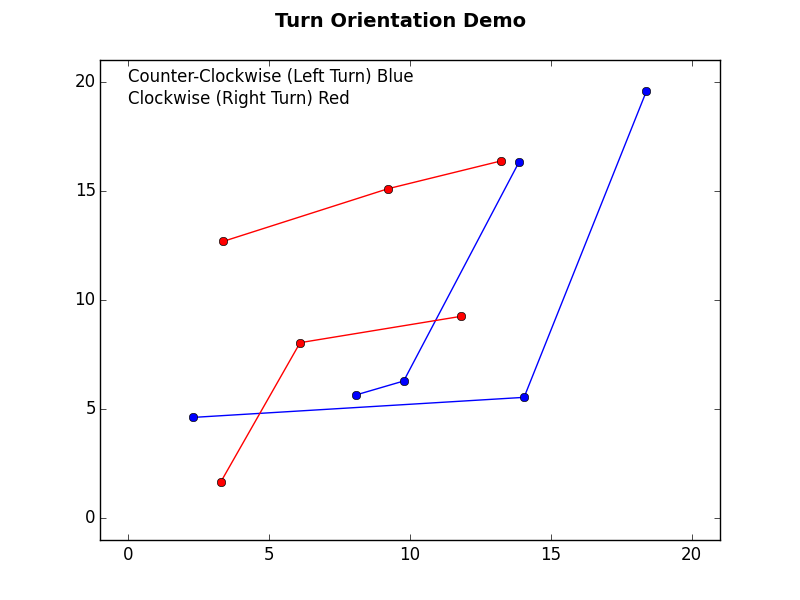
\includegraphics[scale=.4]{turn_orientation.png}}

\subsection{Convex Hull}
\indent With just a one tool in our geometry toolbox, we can solve a fundamental problem of computational geometry - computing the \textbf{convex hull} of a set of points $X$. A convex hull is defined as the minimal subset of points that envelop $X$, or more formally, the intersection of all convex sets containing all $X$. There are well many well-known algorithms, but the one of interest is the Graham Scan, which was published in 1972. \newline \\
\centerline{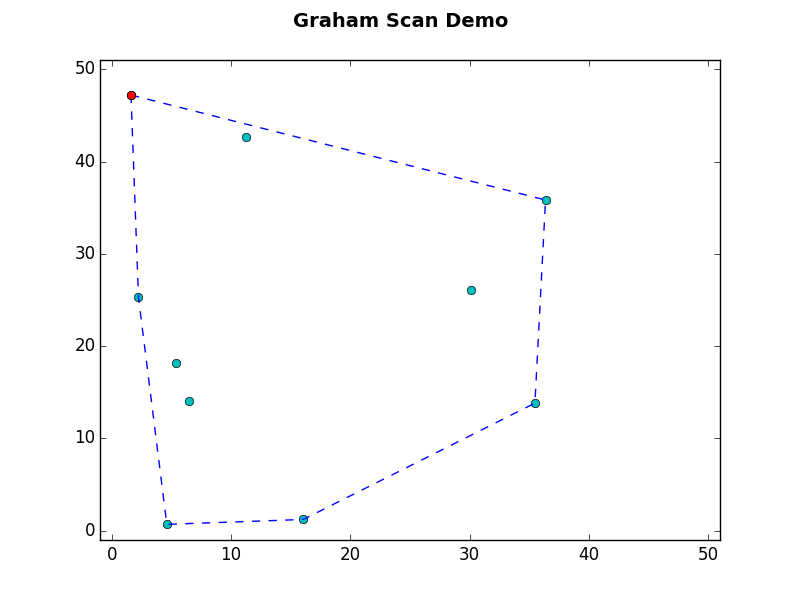
\includegraphics[scale=0.4]{graham_scan.png}}
\indent The algorithm works by splitting the problem into two problems - finding the upper hull and then the lower hull. On a high level, to find the upper hull, we iterate over the points from left to right and have a result set $R$ of points in upper hull. We keep appending points onto our result set and then check to see if the last points make a right turn. If they do not, we know the middle point is not a part of our final result set and we delete the middle point from the result set. We continue this until there are less than 3 points to make a turn, or the last three points do make a right turn. When the algorithm reaches the rightmost point, it terminates and returns the upper hull. The lower hull is computed using the same concept, but all the points in the lower hull will make left turns. \newline \\
\indent If we assume the list of points $P$ is sorted by increasing x coordinates, the runtime algorithm is $O(n)$ where $n = |P|$, as the algorithm will iterate over the list once for each hull - upper and lower. Otherwise, if the list of points is not sorted, we will have to do so and that will be the dominating time complexity of $O(n\ log\ n)$.  The pseudocode for the algorithm is as follows. \newline \\
\begin{algorithm}[H]
\caption{Upper Convex Hull}
\SetAlgoLined
\KwData{P = \{$v_1, v_2, ..., v_n$\}}
\KwResult{the convex hull R}
Sort $P$ by x-coordinate\;
Add $p_1$, $p_2$ to $R$\;
\For{i from 3 to n}{
	Add $p_i$ to $R$\;
	\While{$r_{n-2},\ r_{n-1},\ r_n$ make a left turn}{
		Remove $r_{n-1}$ from $R$\;
	}
}
\Return $R$\;
\end{algorithm}
\vspace*{3ex}
With this algorithm, we have to be careful in certain cases. In the case we have a triple of colinear points on the hull, our algorithm should not include the middle point as the convex hull is defined as the minimal set of points. However, we can fix this relatively easy by ensuring our function that checks right turns returns false if the points are colinear, that is, if the determinant is zero or less.
\subsection{Minkowski Sum}
\indent Once we have understood the concept of a convex hull, we can move onto to an application of the convex hull. Once we have the convex hull of two polygons, we can see if they collide. The \textbf{minkowski sum} of two vectors $S_1 \subset \mathbb{R}$ and $S_2 \subset \mathbb{R}$ is defined as $S_1 \oplus S_2 = \{p_x + q_x,\ p_y + q_y : p \in S_1,\ q \in S_2\}$. Similarly, the \textbf{minkowski difference} is defined as $S_1 \ominus S_2 = \{p_x - q_x,\ p_y - q_y : p \in S_1,\ q \in S_2\}$. Two polygons intersect in $\mathbb{R}^2$ if and only if $(0,\ 0) \in S_1 \ominus S_2$. With Minkowski differences, we can extend this collision detection to an arbitrary amount of dimensions, checking to see if the zero vector lies within the Minkowski difference.
\centerline{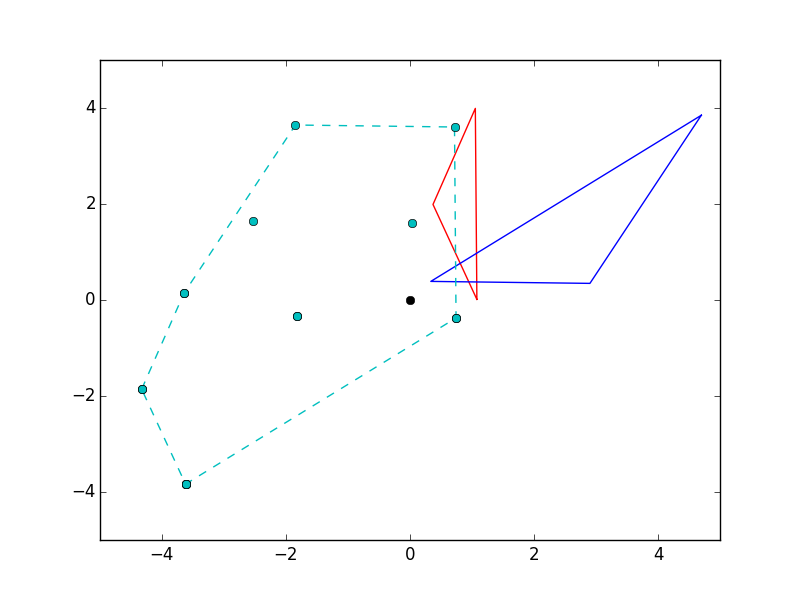
\includegraphics[scale=0.4]{minkowski_colliding.png}} 
\indent Computing the Minkowski sum of two sets $S_1,\ S_2$ has a naive implementation of $O(n^2) + O(n\ log\ n)$, the addition of every point with another, followed by the calculating of the convex hull, but we can do better we have some constraints on the types of polygons given. If we consider an edge of $S_1 \oplus S_2$, we say the edge is \textbf{extreme}, that is, it has to be generated by points of $S_1, S_2$ that are extreme in this same direction. This way, each edge in $S_1, S_2$ is \textbf{charged} at most once.
\centerline{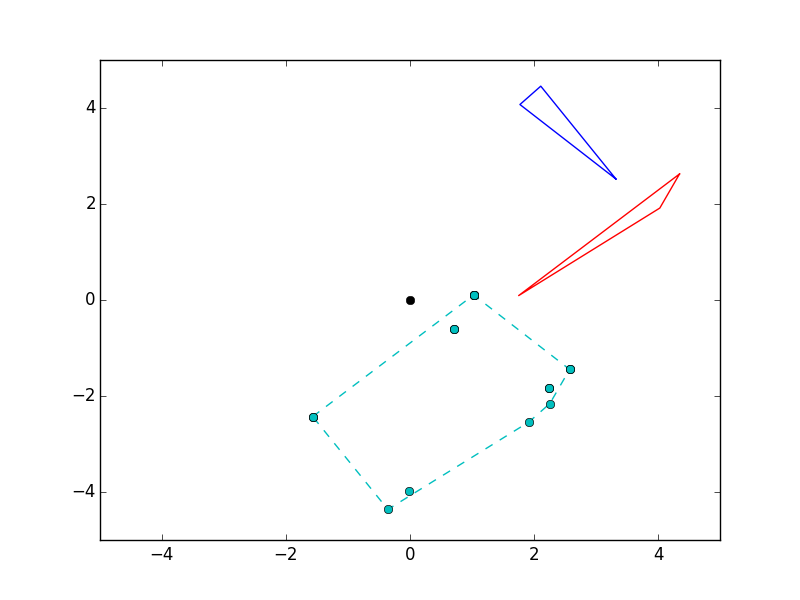
\includegraphics[scale=0.4]{minkowski_noncolliding.png}}
\textbf{Theorem 13.11 (DeBerg)} The tight bound of calculating the Minkowski Sums are as follows \newline \\
(1) $\theta(n+m)$ \emph{if both polygons are convex}. \newline
(2) $\theta(nm)$ \emph{if one polygon is convex and the other is concave}. \newline
(3) $\theta(n^2m^2)$ \emph{if both polygons are concave}. \newline \\
\indent The major application of Minkowski sum is in collision detecting. For instance, in robot motion planning, the robot and obstacles are represented by convex set of points and we can use the Minkowski sum to plan the motion of the robot by computing the \textbf{forbidden space} of the robot. \newline \\
\begin{algorithm}[H]
\caption{Minkowski Sum}
\SetAlgoLined
\KwData{P = \{$v_1, v_2, ..., v_n$\}, \newline R = \{$w_1, w_2, ..., w_m$\}}
\KwResult{the vertices of $P \oplus R$}
$i \leftarrow 1$; $j \leftarrow 1$\;
$v_{n+1} \leftarrow v_1$; $v_{n+2} \leftarrow v_2$\;
$w_{m+1} \leftarrow w_1$; $w_{m+2} \leftarrow w_2$\;
\While{true}{
	Add $v_i + w_j$ to $P \oplus R$\;
	\If{$angle(v_i, v_{i+1}) < angle(w_j, w_{j+1})$}{
		$i \leftarrow i + 1$\;		
	}
	\ElseIf{$angle(v_i, v_{i+1}) > angle(w_j, w_{j+1})$}{
		$j \leftarrow j + 1$\;
	}	
	\Else{
		$i \leftarrow i + 1$;	 $j \leftarrow j + 1$\;
	}
}
\Return $P \oplus R$\;
\end{algorithm}

\subsection{Triangulations}
\indent The \textbf{Art Gallery Problem} is defined as follows, given a room of various shape, how many cameras are needed to guard it? We can add some restrictions to the shape of the room, that the room will be a \textbf{simple polygon}, which is defined as a region closed that does not intersect itself. When we approach this problem, the Art Gallery Problem is essentially asking for the \textbf{triangulation} of the room - how many pieces are required to decompose this polygon into a set of triangles? \newline \\
\indent Triangulation of a polygon takes quadratic time in the worst case and is implemented recursively. We start from a point, find a diagonal, and call this recursively on the remaining points of the polygon. Finding a diagonal takes linear time as we check the leftmost vertex of $P$ and try to connect its two neighbors $u$ and $w$; if this fails we connect $v$ to the vertex farthest from $\overline{uw}$ inside the triangle defined by $u$, $v$, and $w$. \newline \\
\centerline{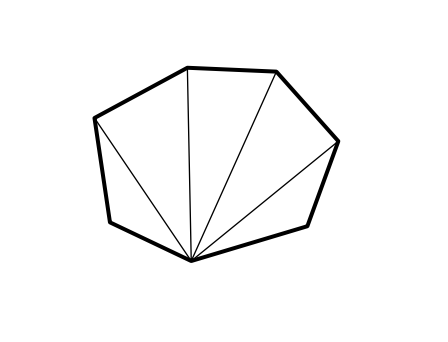
\includegraphics[scale=0.4]{convex_triangulation.png}}
\indent Given a convex polygon, we can triangulate this in linear time - simply pick a vertex and draw a diagonal line to every other vertex besides its direct neighbors. So the main challenge is decomposing a simple polygon into a set of convex polygons and we can see an easier approach is to decompose the polygon into \textbf{monotone polygons}. A simple polygon is monotone with respect to a line $l$ if for any line $l'$ perpendicular to $l$, the intersection is connected.
\subsection{Internal Coordinates}
\indent A common way to represent molecules is to simply write the Cartesian coordinates of each atom. The standard form is \textbf{Protein Data Bank (PDB)} in which each row represents an atom and contains coordinates and other data. Another way to represent molecules is with \textbf{internal coordinate representation} or \textbf{Z-matrix}. In this representation, the molecule consists of each atom by its relative position to other neighbors atoms. This includes bond length, bond angle, and dihedral angle - the angle between the planes between a triple of atoms. \newline \\
\indent The task given by Nathan was to convert PDB files into a Z-matrix form. I had spent about two weeks doing this manually with a Python script, using a molecular library called \textbf{MolMod} to parse the PDB files and had completed the PDB to Z-matrix, and then, when starting the Z-matrix back to PDB and looking through various algorithms to reconstruct this, I found in the \textbf{oBabel} documentation that this was included within oBabel. \newline \\
\indent The motivation behind this task is to validate 3-dimensional structures of proteins. With a typical representation of molecules in cartesian space, the amount of search space is a significant factor larger than that of internal coordinates. 
\subsection{VolRover}
\indent The most recent task assigned was to help develop a functionality of \textbf{VolRover}. Given a set of png files of neuron forests with unique colors per item, generate an xml file of the resulting contours, labeled with a unique id that is consistent throughout the several images. For each set of images, we will generate a series file with some metadata and for each particular image, there is to be a trace file, in xml format, of the contours. From these trace files, we can reconstruct the the 3d image of the neuron forests.
\end{multicols}
\end{document}
